%%-*-latex-*-

\section{Software}

\begin{figure}
  \centering
  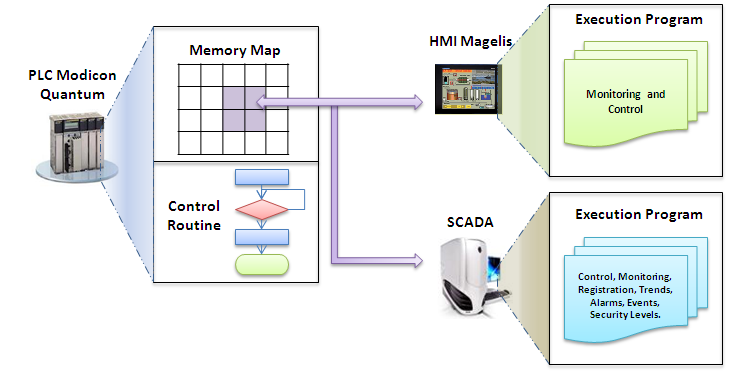
\includegraphics[width=0.5\textwidth]{img/software.png}
  \caption{Software interaction schema}
  \label{fig:software}
\end{figure}

The entire system development involved programming the Quantum PLC,
the HMI application and the SCADA software which is the automation's
main component. \Fig{fig:software} shows the schema of how the programs are
executed within each component. It is observed the interaction between
the PLC software trough a memory map used to read and write data
inside both the HMI and the SCADA. Intuitively, it is noted the
concept behind the automation system workings. Here, the SCADA or the
HMI writes a data at the PLC's memory map in order to execute a
command when a new control routine cycle begins.

\begin{figure}
  \centering
  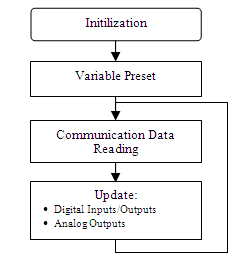
\includegraphics[width=0.2\textwidth]{img/plc.png}
  \caption{PLC routine blocks diagram}
  \label{fig:plc}
\end{figure}

The PLC software routine is developed at Ladder over Structured Text
because of its function within the system. The block diagram
represented by this routine is show in \fig{fig:plc}. In this diagram,
when the PLC begins the variables values are defined and preset. Immediately, the
reading of data is done trough the specified communication channels,
internally, the arithmetic operations for data conversion are also
executed and finally, the digital outputs and inputs and analog
outputs are updated. With this, a new operation cycle is started
obtaining a reliable execution and an efficient data update.

The Vijeo Designer software native to the Magelis Smart tactile
screens has been used for the programming of the HMI at the
Cantagallo generation center. The final application has interactive
menus to navigate, hardware control and supervision screens, security
access levels for users, tendencies graphs and a registry of active
and historic alarms. A  general view of the interface is shown in
\fig{fig:hmi}. For simplicity the operation of HMI is similar to the SCADA.

\begin{figure}
  \centering
  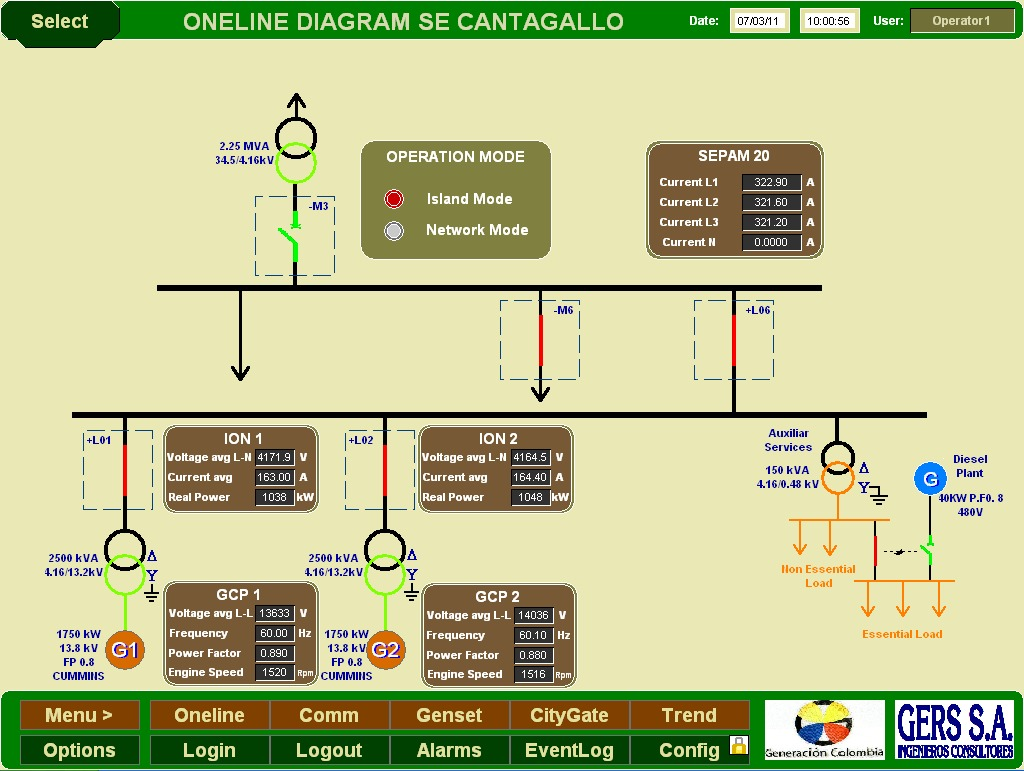
\includegraphics[width=0.5\textwidth]{img/hmi.png}
  \caption{Cantagallo Human-Machine Interface}
  \label{fig:hmi}
\end{figure}

The one-line diagram shows the HMI and the complete information
presented to the operator. Similarly the control schema are shown for
each generation bay and the supervision data are collected in a set of
screens for machines' electrical and mechanical data.

\begin{figure}
  \centering
  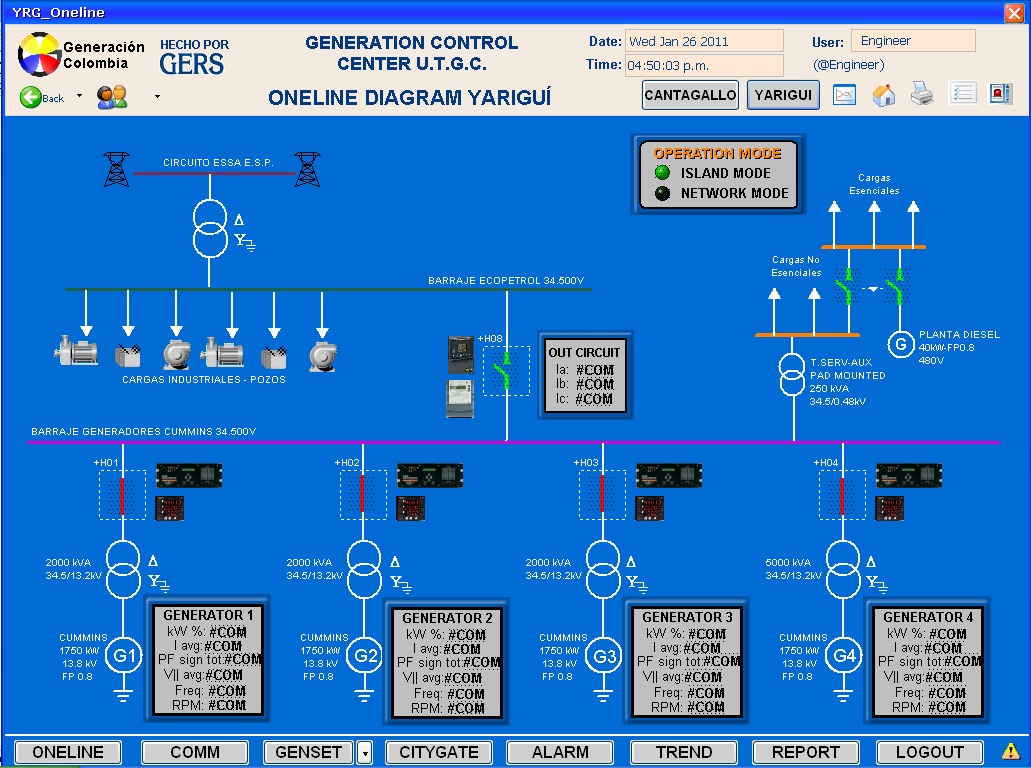
\includegraphics[width=0.5\textwidth]{img/oneline_scada.png}
  \caption{SCADA Vijeo Citect, Yariguí power plant one-line diagram}
  \label{fig:onelinescada}
\end{figure}

\begin{figure}
  \centering
  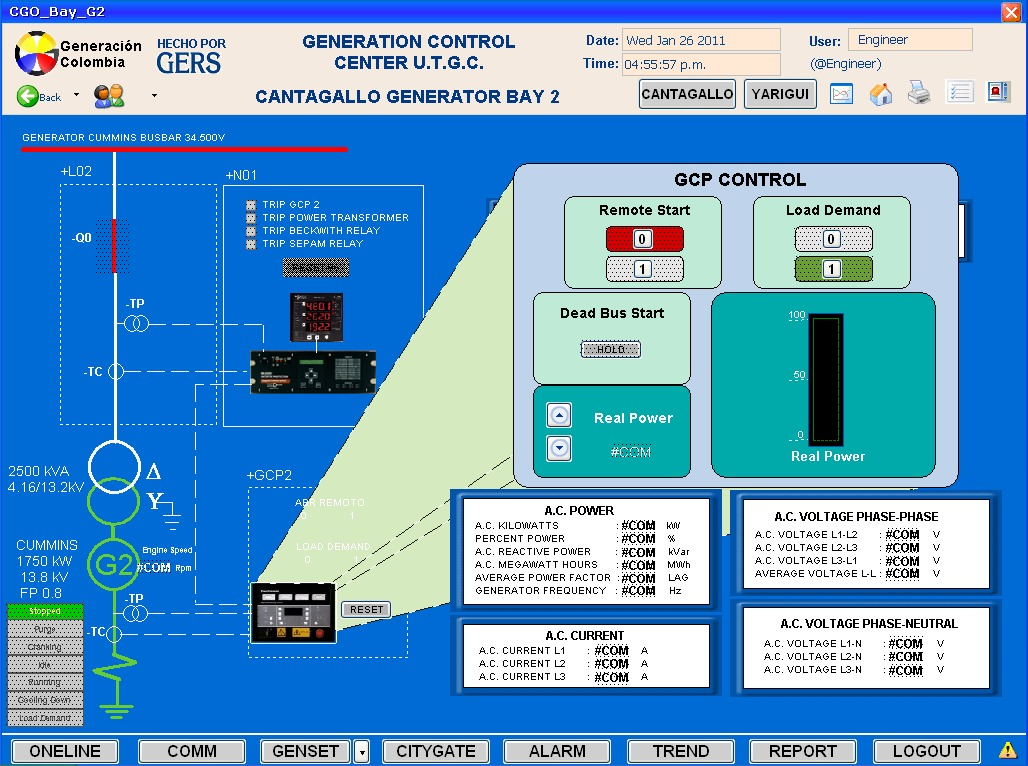
\includegraphics[width=0.5\textwidth]{img/bay_scada.png}
  \caption{SCADA Vijeo Citect, Control schema for Cantagallo power plant bay 2}
  \label{fig:bayscada}
\end{figure}

The characteristics programmed in the SCADA Vijeo Citect offer
supervision and control screens for each bay, besides of reports
generation, alarm informs, tendencies graphs, security records,
communication link status for damage reports. Every one of them
under the requirements initially expressed. \Fig{fig:onelinescada}
shows the running SCADA where the operation centers might be operated.

Bay control can be seen in \fig{fig:bayscada}, it offers every electrical
and mechanical data needed to operate the generators. They include:
start, stop, deadbus closure and the power variation given by the
generator during network mode (synchronization of the generation
center with the public electrical network). Additionally it shows the
reset for the several hardware in case of failure or trip and for the
synchronization of the generation centers with the network, the trip
in case of return to island mode and the opening and closing of the
output switch.

The gas meter data is integrated into the SCADA informing the operator
of the generator's gas input conditions. This functionality is vital
for being the gas the machine's combustible. The alarms screen has a
registry of active alarms, summarize and hardware alarms. Every alarm
has a priority level and a category used to generate a sound according
to the urgency. The tendencies screen offers to the operator the
capacity of viewing each variable of the generation center with data
store for as long as one year. It also offers ease of visualization
with capabilities like change of axis and scale. The following reports
can be generated: events, control operations made by every operator,
security access to the SCADA and a report of every alarm generated
during the previous year. Finally, security plays an important role on
every supervision and control system, to guarantee this, several access
levels have been created, including every system user such as operator,
engineer or administrator.
